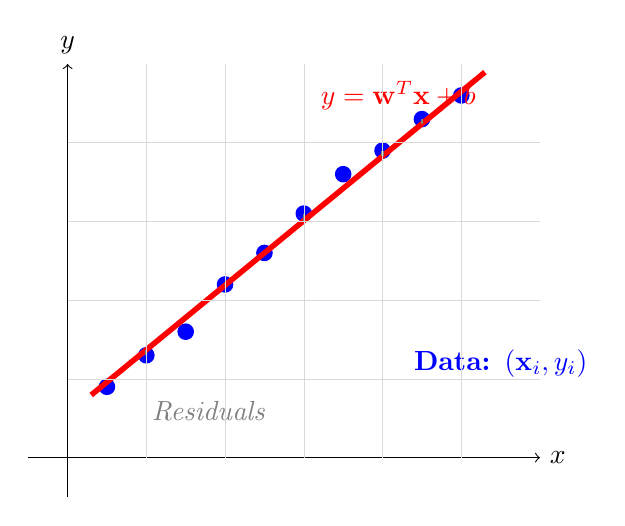
\begin{tikzpicture}[scale=1.0]
  \draw[->] (-0.5,0) -- (6,0) node[right] {$x$};
  \draw[->] (0,-0.5) -- (0,5) node[above] {$y$};
  
  % More realistic data points with slight scatter
  \foreach \x/\y in {0.5/0.9, 1/1.3, 1.5/1.6, 2/2.2, 2.5/2.6, 3/3.1, 3.5/3.6, 4/3.9, 4.5/4.3, 5/4.6} {
    \fill[blue] (\x, \y) circle (3pt);
  }
  
  % Regression line - thicker
  \draw[thick, red, line width=2pt, domain=0.3:5.3] plot (\x, {0.82*\x + 0.55});
  \node[red] at (4.2, 4.6) {$y = \mathbf{w}^T\mathbf{x} + b$};
  
  % More visible residuals
  \draw[dashed, gray, thick] (1, 1.3) -- (1, 1.37);
  \draw[dashed, gray, thick] (2, 2.2) -- (2, 2.19);
  \draw[dashed, gray, thick] (3, 3.1) -- (3, 3.01);
  \draw[dashed, gray, thick] (4, 3.9) -- (4, 3.83);
  \draw[dashed, gray, thick] (4.5, 4.3) -- (4.5, 4.24);
  
  % Better labels
  \node[blue] at (5.5, 1.2) {\textbf{Data: $(\mathbf{x}_i, y_i)$}};
  \node[gray] at (1.8, 0.6) {\textit{Residuals}};
  
  % Grid for better readability
  \foreach \x in {1,2,3,4,5} {
    \draw[very thin, gray!30] (\x, 0) -- (\x, 5);
  }
  \foreach \y in {1,2,3,4} {
    \draw[very thin, gray!30] (0, \y) -- (6, \y);
  }
\end{tikzpicture}
